\chapter{Introduction}
\label{chap:intro}



\begin{figure*}[b]
\centering
 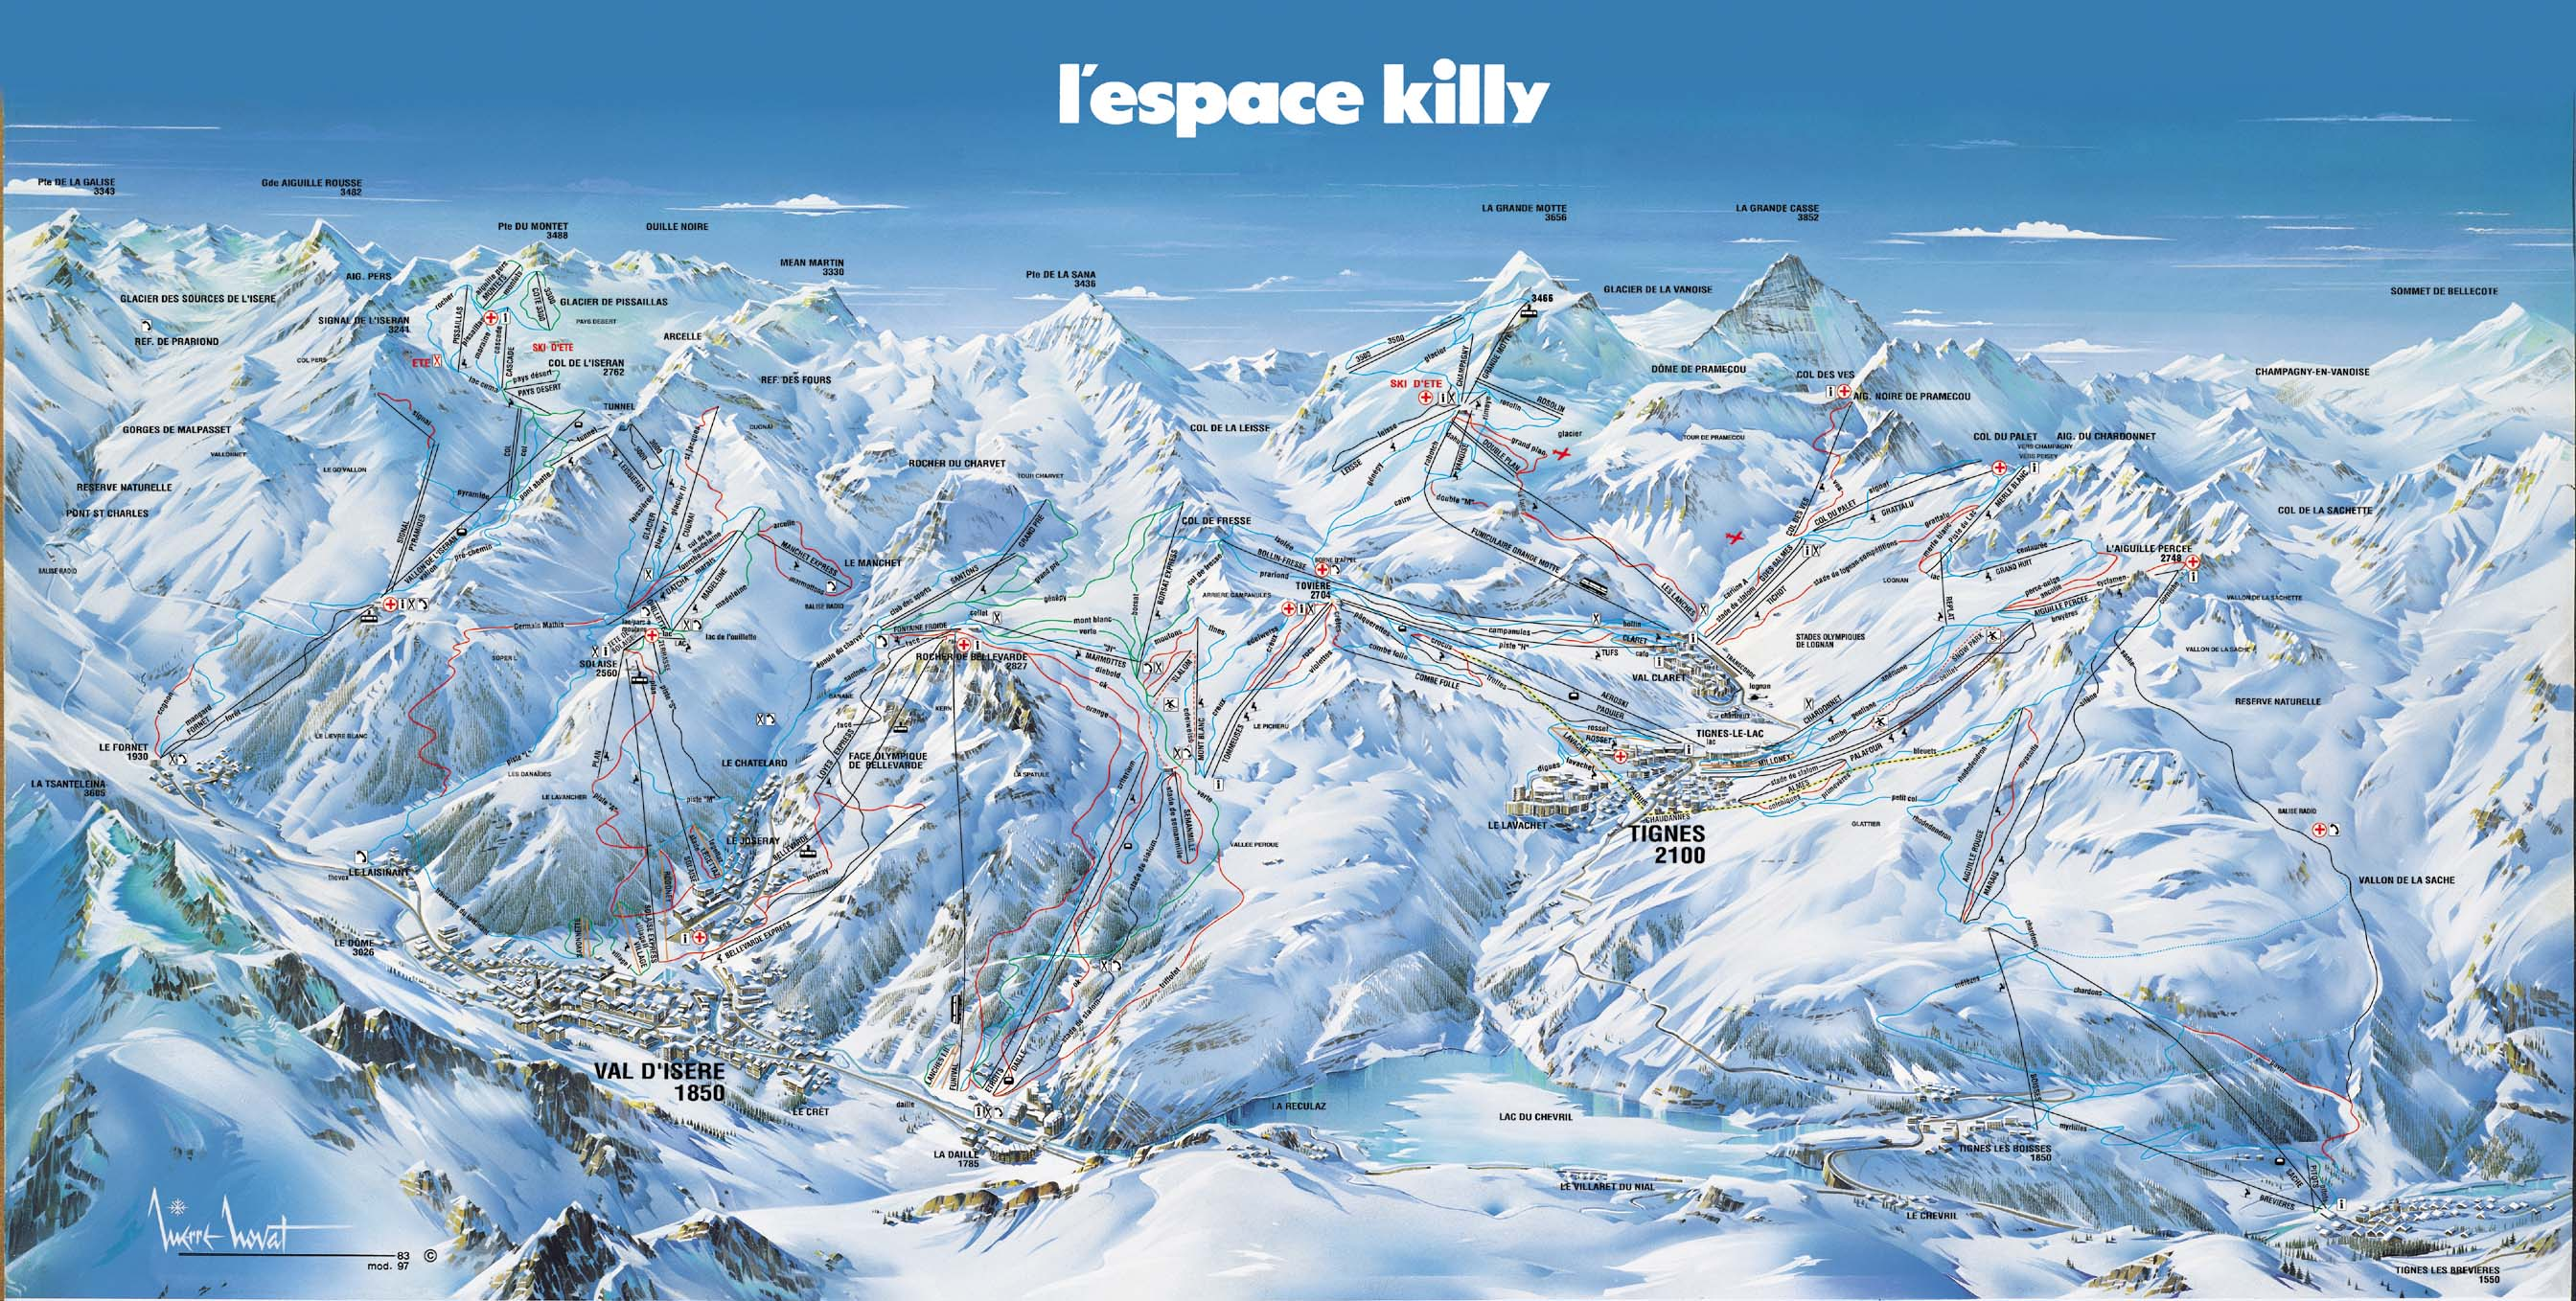
\includegraphics[width=1.0\linewidth]{novat/PN_killy.jpg}
 \caption{\label{killy} Espace Killy (Val D'Isere, Tignes) par Pierre Novat}
\end{figure*}

 Un panorama est une représentation visuelle grand angle d'un espace physique. Cette image, prise d'un point de vue particulier, généralement surélevé, permet d'avoir une vue d'ensemble sur une région donnée. C'est une œuvre artistique, où l'artiste, en photo, en peinture ou en dessin peut choisir de mettre en avant certains éléments au détriment d'autres. Les cartes panoramiques sont des panoramas particuliers ayant pour but de servir de carte à un utilisateur non-expert. En effet la vue dégagée d'un panorama permet de se repérer et de s’orienter. De plus les artistes qui créent ces panoramas sont aussi des experts en cartographie. Seulement, la création de panorama est un processus long et compliqué et le savoir-faire commence tout doucement à se perdre avec l'arrivée des outils informatiques qui permettent la création rapide de cartes. Cependant ces cartes ne sont pas de la même qualité que les cartes panoramiques faites par des artistes qui vont toujours chercher à faire aimer la région qu'ils représentent en prenant en considération des éléments autres que géographiques. Ainsi vient la question de l'automatisation des panoramas en essayant de produire un résultat proche de ce que pourrait produire un artiste. C'est un objet d’étude intéressant pour une recherche sur la question de la stylisation de modèles 3D car les panoramas posent de façon cruciale la question de comment et quoi représenter pour une application très spécifique : permettre une lecture utile et esthétique du paysage. C’est aussi un cas d’étude permettant d’explorer la marge de manœuvre à laisser au designer dans le processus de création : un  compromis à faire entre contrôle et automatisation.
 
Dans notre coté, nous nous intéressons au rendu de panorama de montagnes, plus particulièrement dans le style de l'atelier Pierre Novat (Fig. \ref{killy}). Pour comprendre le processus de création de ces panoramas, nous avons travaillé avec l'aide d'Arthur Novat. Cette collaboration nous a permis d'expliciter un ensemble de règles qu'il utilise pour la création de ses panoramas pour pouvoir ensuite les traduire en algorithme pour produire un rendu dans le style Novat. Nous nous sommes plus spécifiquement intéressés au calcul d'un ombrage qui donne à voir le relief d'un terrain montagneux et pourra servir de base au dessin d'un panorama. 

Dans ce rapport, nous présentons dans un premier temps notre étude sur le style des panoramas de Pierre Novat  pour comprendre comment chaque élément est construit, notamment les ombres et la lumière. Dans un second temps nous étudions la manière qu'ont les cartographes de dessiner les ombres et les précédents travaux en informatique graphique sur les ombres, en particulier \textit{exagerated shading} \cite{rusinkiewicz2006exaggerated} qui propose un ombrage orienté vers la cartographie. Ensuite nous présentons notre solution pour calculer un ombrage expressif construit à l'aide des précédentes études et des règles que nous avons produites. Enfin nous montrons notre méthode de validation et les travaux futurs. 


\begin{figure*}[h!]
\centering
 \begin{subfigure}[t]{0.49\linewidth}
   \centering
   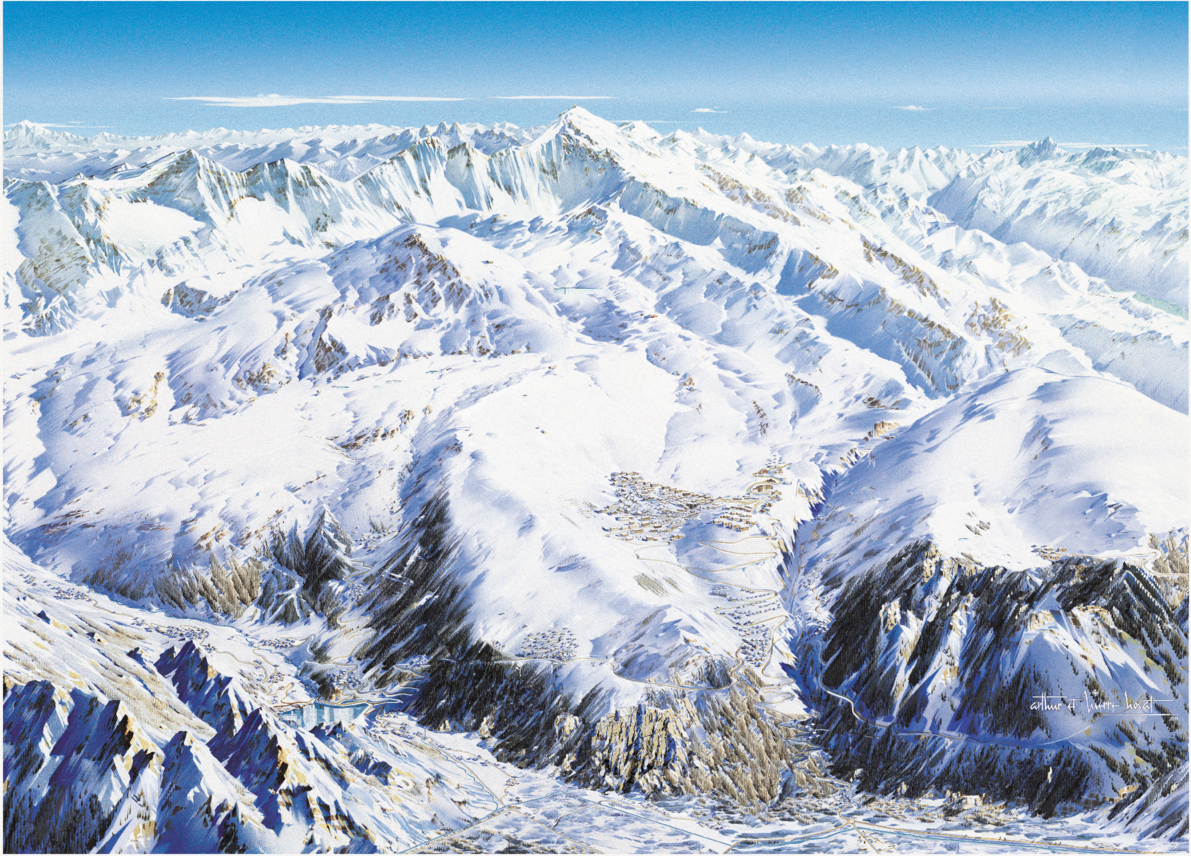
\includegraphics[width=1.0\linewidth]{novat/AlpeHuez.png}
   \caption{Sans les pistes}
 \end{subfigure}
 \begin{subfigure}[t]{0.49\linewidth}
   \centering
   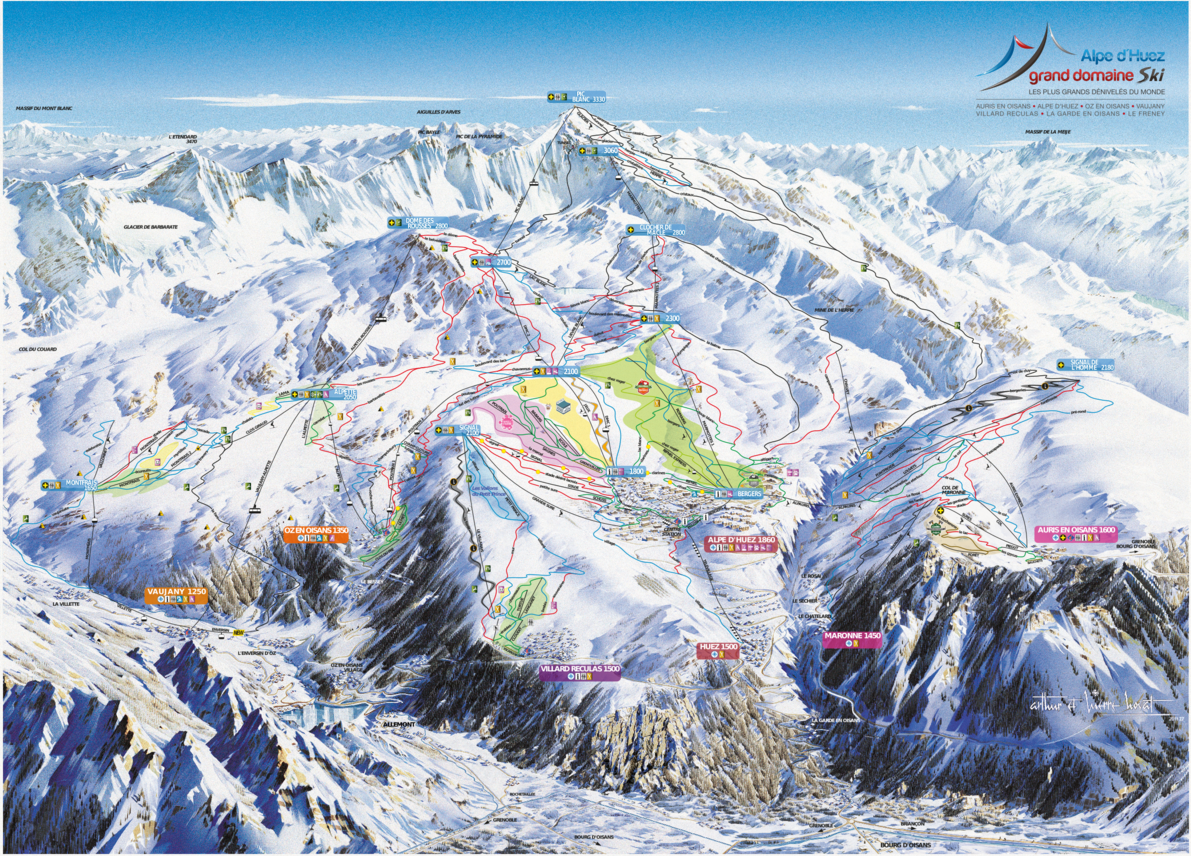
\includegraphics[width=1.0\linewidth]{novat/AlpeHuez_pistes.png}
   \caption{Avec les pistes}
 \end{subfigure}
 \caption{L'Alpes d'Huez par Arthur et Pierre Novat}
\end{figure*}
